\section{Punto de Vista de Migración}
\subsection{Modelo de Migración}
\begin{figure}[h!]
	\centering
	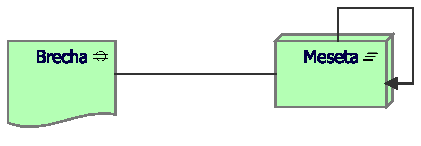
\includegraphics[width=.9\linewidth]{imgs/modelo/Migracion.pdf}
	\caption{Modelo Migración}
\end{figure}
El punto de vista de la migración implica modelos y conceptos que se pueden utilizar para especificar la transición de una arquitectura existente a una arquitectura deseada.

\subsection{Caso  de Migración}
\begin{figure}[h!]
	\centering
	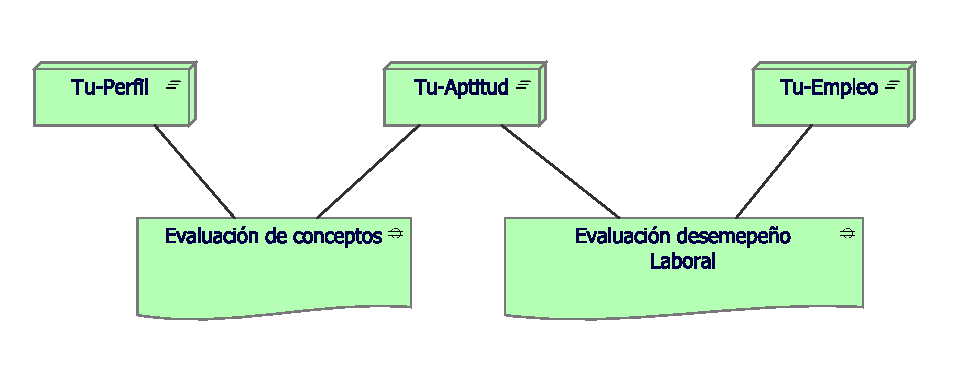
\includegraphics[width=.9\linewidth]{imgs/caso/proyecto/migracion.pdf}
	\caption{Caso Migración}
\end{figure}
En el punto visto de migración para el caso de estudio se plantea la aplicación inicial de Tu-Perfil que permitirá el perfilamiento y acompañamiento del estudiante. Como Siguiente versión se pretende implementar una aplicación (Tu-Aptitud) que evalúe de manera estricta los conceptos adquiridos durante la formación vocacional del estudiante y así lograr concebir las aptitudes más sobresalientes que ayudarán a encaminar a el estudiante a la vida profesional buscando ser apto según estas aptitudes. El siguiente paso es la construcción de una aplicación(Tu-Empleo) que evalúe el desempleo del profesión en la vida laboral, logrando establecer sus fortalezas y debilidades, además de inducir a la persona evaluada en la posibilidad no de cambiar de ambiente  laboral.